%!BIB TS-program = biber
\documentclass[11pt]{article}%
\usepackage{amsmath}
\usepackage{amsfonts}
\usepackage{amssymb,tcolorbox}
\usepackage{graphicx}
\usepackage{amssymb}%
\usepackage{siunitx}
\usepackage{listings}
\usepackage{float}
\usepackage[style=ieee]{biblatex}
\setcounter{MaxMatrixCols}{30}
\providecommand{\U}[1]{\protect\rule{.1in}{.1in}}
\providecommand{\U}[1]{\protect\rule{.1in}{.1in}}
\providecommand{\U}[1]{\protect\rule{.1in}{.1in}}
\newtheorem{theorem}{Theorem}
\newtheorem{acknowledgement}[theorem]{Acknowledgement}
\newtheorem{algorithm}[theorem]{Algorithm}
\newtheorem{axiom}[theorem]{Axiom}
\newtheorem{case}[theorem]{Case}
\newtheorem{claim}[theorem]{Claim}
\newtheorem{conclusion}[theorem]{Conclusion}
\newtheorem{condition}[theorem]{Condition}
\newtheorem{conjecture}[theorem]{Conjecture}
\newtheorem{corollary}[theorem]{Corollary}
\newtheorem{criterion}[theorem]{Criterion}
\newtheorem{definition}[theorem]{Definition}
\newtheorem{example}[theorem]{Example}
\newtheorem{exercise}[theorem]{Exercise}
\newtheorem{lemma}[theorem]{Lemma}
\newtheorem{notation}[theorem]{Notation}
\newtheorem{problem}[theorem]{Problem}
\newtheorem{proposition}[theorem]{Proposition}
\newtheorem{remark}[theorem]{Remark}
\newtheorem{solution}[theorem]{Solution}
\newtheorem{summary}[theorem]{Summary}
\newenvironment{proof}[1][Proof]{\noindent\textbf{#1.} }{\ \rule{0.5em}{0.5em}}
\addtolength{\oddsidemargin}{-.875in}
\addtolength{\evensidemargin}{-.875in}
\addtolength{\textwidth}{1.75in}
\addtolength{\topmargin}{-1in}
\addtolength{\textheight}{2in}
\usepackage{tocloft}
\usepackage{color} %red, green, blue, yellow, cyan, magenta, black, white
\definecolor{mygreen}{RGB}{28,172,0} % color values Red, Green, Blue
\definecolor{mylilas}{RGB}{170,55,241}

\addbibresource{report.bib}

\title{MANE 6710 - Numerical Design Optimization Lab 3}
\author{Human 6966}
\date{November 15 2024}

\renewcommand{\contentsname}{Table of Contents:}
\setcounter{tocdepth}{2} % Include sections and subsections
\setlength{\cftbeforesecskip}{0.5cm} % Adjust spacing between entries
\begin{document}
\maketitle
\newpage
\tableofcontents
\newpage
\addcontentsline{toc}{section}{Executive Summery}
\section*{Executive Summery}
\label{sec:abstract}

Tilt-A-Whirls are a common and beloved small-town fair ride suitable for children and adults alike. Their fun comes from the random changes in the spin direction of the cart the rider is in as the ride goes over a hilly track. This behavior is due to the chaotic dynamics of the underdamped double pendulum that governs the ride's dynamics. The task of this lab is to maximize the chaotic nature of the ride by setting the second arm length, speed, and hill size using a surrogate model based optimization scheme in Matlab. The dynamics of the ride are analyzed through a non-dimentionalized equation from a paper by R. L. Kautz and B. M. Huggard. The GPLM surrogate model optimized by \lstinline{fmincon()} was successfully  able to maximize the standard deviation of the cart's angular velocity at state conditions.

\section{Analysis Introduction}
\label{sec:intro}

\subsection {Methodology}
\label{sec:analysismethod}

The dynamics model used for the behavior of the Tilt-A-Whirl is given on the 63rd page of “Chaos at the amusement park: Dynamics of the Tilt-A-Whirl” by R. L. Kautz and B. M. Huggard and is shown in equation \ref{eqn:dynamics} \cite{dynamics}.

\begin{equation}
\label{eqn:dynamics}
\frac{d^{2}\phi}{d\tau^{2}}+\frac{\gamma}{Q_{0}}\frac{d\phi}{d\tau}+(\epsilon-\gamma^{2}\alpha)\sin(\phi)+\gamma^{2}\beta\cos(\phi)=0
\end{equation}

With:
\begin{enumerate}
	\item $\phi$ being the angular position of the center of mass about the axis of rotation of the cart
	\item $\tau$ being nondimensional time
	\item $Q_{0}$ being the energy dissipation ratio of the cart per rotation
	\item $\epsilon=\frac{r_{1}}{9r_{2}}$
	\item $\alpha =\alpha_{0}-\alpha_{1}*\cos(\tau)$
	\item $\beta=3\alpha_{1}\sin(\tau)$
	\item $\gamma=\frac{\sqrt{g}}{3\omega\sqrt{r_{2}}}$
	\item $r_{1}$ being the radius between the ride's and cart's axies of rotation
	\item $r_{2}$ being the radius between the center of mass and the axis of rotation of the cart
	\item $\alpha_{0}$ being the initial slope of the hills
	\item $\alpha_{1}$ being the incline angle of the hills
	\item $g$ being gravitational acceleration constant (9.81 m/s/s)
	\item $\omega$ being the angular velocity of the ride about its axis of rotation
\end{enumerate}

Equation \ref{eqn:dynamics} is converted into the state space representation given in equation \ref{eqn:state} so the equation could be solved using Matlab's \lstinline{ode45()} function.

\begin{equation}
\label{eqn:state}
\dot{\vec{\phi}}= \left[\begin{array}
[c]{c}
\dot{\phi_{1}}\\
\dot{\phi_{2}}\end{array}\right] = \left[\begin{array}
[c]{c}
\phi_{2} \\
 -1(\frac{\gamma}{Q_{0}}\phi_{2}+(\epsilon-\gamma^{2}\alpha)\sin(\phi_{1})+\gamma^{2}\beta\cos(\phi_{1}))
 \end{array}\right]
 \end{equation}

With states $ \phi_{1}=\phi$ and $\phi_{2}=\frac{d\phi}{d\tau}$ (Note the .-1 was factored out of the second state equation to reduce the error of the floating point math as it would accumulate and affect results). This state space system can be solved using a nonlinear differential equation solver like \lstinline{ode45()}, the results of which can be used in the objective function using equation \ref{eqn:obj}.

\begin{equation}
\label{eqn:obj}
\sigma_{\dot{\phi}} = -3\omega\sqrt{\frac{\int_{0}^{T}(\phi_{2}-\bar{\phi_{2}})^{2}d\tau}{T}}
\end{equation}

Where: 
\begin{enumerate}
	\item $T$ is the nondimensional period of the ride 
	\item $\sigma_{dot{phi}}$ is the standard deviation of the cart's angular velocity
	\item $\bar{\phi_{2}}=\frac{\int_{0}^{T}\phi_{2}d\tau}{T}$
\end{enumerate}

Note that since Matlab's \lstinline{fmincon()} is a minimization function and the task is to maximize the standard deviation of the cart's angular velocity, the objective equation (equation \ref{eqn:obj}) results in -1* the standard deviation of the cart's angular velocity. Additionally Matlab's \lstinline{trapz()} was used to compute the numerical integration.

\subsection{Assumptions}
\label{sec:assumption}
To simplify the physical model and fundamental equations, the following assumptions were made:
\begin{enumerate}
   	 \item $Q_{0}$, the term that accounts for mass and friction, has a constant value of 20
   	 \item Negligible air resistance
   	 \item The ride's structure is rigid enough to support any rider(s) with negligible transient effects on ride performance
   	 \item The beam length from the center of the ride to the center of rotation of the carts ($r_{1}$) is 4.3 meters
   	 \item $r_{2}$ is constant (the rider(s) have a negligible impact on center of mass)
   	 \item The incline offset $\alpha_{0}$ is 0.036 radians
   	 \item Neglect effects from manufacturing and wear on system values
   	 \item Given a long enough period, any realistic initial conditions will have negligible effects on the dynamics
   	 \item Small angle approximation
\end{enumerate}


\subsection{Limitations}

These assumptions limit this analysis method by neglecting the effect the rider(s), external forces, and transient structural behaviors have on the system's dynamics. This is important as the ride's dynamics are chaotic in nature meaning that small changes in inputs can potentially have significant impacts on the system's behavior over time. Thus it is important to note that experimental results that include the neglected factors will show behavior that deviates from the model. Additionally, this model might miss a more optimal design that comes from including these factors. Finally, by assuming constant $r_{2}$, the analysis is limited to cases where the rider(s) are still, have the same mass, and sit in the same place (which is rarely the case).

\section{Optimization Method and Limitations}
\label{sec:optimizationmethod}

The optimization method chosen for this project was surrogate model based optimization. This is due to the high level of noise in the objective function as \lstinline{fmincon()} is highly sensitive to sharp peaks and thus struggles with chaotic functions. The surrogate model was chosen to have a fifth-order isometric Matern covariance function (because it handles noisy functions with nonsimilar length scales better than other options like a Gausian radial basis function) with a Gausian likelihood function. To build the model, the Latin-Hypercube sampling method was employed to get the value of the objective function at 200 points distributed across the bounded design space. From these samples and an initial guess for the hyperparameters (see section \ref{sec:results}), the likelihood function was maximized to optimize the hyperparameters of the surrogate model and the surrogate model was minimized using \lstinline{fmincon()}.

The SQP (Sequential Quadratic Programming) Algorithm was chosen for \lstinline{fmincon()} (Matlab's nonlinear optimization problem solver \cite{matlab}) to solve the minimization problem. The SQP algorithm uses a quasi-Newton update method to approximate the Hessian, which is used to solve the quadratic subproblems with the constraints and model linearized around the current state. Then the algorithm does a line search to determine the step size in the direction of the solution for the generalized model. The algorithm iterates through the updated states until a local minimum of the generalized model is found. To perform this analysis, the following assumptions were made:

\begin{enumerate}
	\item Constraints are continuously twice differentiable
	\item The objective function is continuously twice differentiable
	\item There is a `good' initial guess
	\item There is a `good' surrogate model
\end{enumerate}

To minimize the error due to the fourth assumption, an update step was used. After \lstinline{fmincon()} converges to a local minimum, the objective function was sampled at that location. If the error between the model and the objective function was greater than $5*10^{-2}$ (which was chosen by incrementally decreasing the tolerance until the condition was no longer met in 500 iterations) the hyperparameter maximization and \lstinline{fmincon()} were rerun with the new sample added to the model.

The methodology and assumptions impose the following limitations on this analysis method:
\begin{enumerate}
	\item Due to the derivative assumptions, smooth surrogate model functions are required
	\item Due to ending conditions, the surrogate model must closely follow the trends of the objective function without violating the smoothness condition
	\item Due to the gradient-driven update method, the solution may not recover from a step outside the constraints
	\begin{itemize}
		\item Initial guess should start solver inside constraints (algorithm may or may not work otherwise)
		\item A 'bad' step can put algorithm outside constraints
	\end{itemize}
	\item The algorithm won't know if the minimum it found is a local or global minimum 
	\item If the objective function behavior cannot be adequately captured in the generalized linear model, then \lstinline{fmincon()} can take ’bad’ steps due to deviation between actual and linearized models
\end{enumerate}

\section{Optimization Problem}
\label{sec:problem}

The objective of this lab is to apply the principles learned in lecture to optimize the user experience on a tilt-a-whirl modeled within the following criteria and constraints \cite{lab3doc}:
\begin{enumerate}
	\item The angular velocity of the ride is to be between 3 rpm and 8 rpm ($3\leq\frac{30\omega}{\pi}\leq8$)
	\item The radial distance between the center of mass and axis of rotation should be between 0.1 and 1.5 meters ($0.1\leq r_{2}\leq1.5$)
	\item The incline angle of the hills should be less than 0.3 rad ($0\leq\alpha_{1}\leq0.3$)
\end{enumerate}
The user experience on a tilt-a-whirl can be optimized by maximizing (or minimizing the negative of) the standard deviation of the rider's angular velocity. To analyze the problem the model's state dynamics were parameterized in terms of the design variables, solved using \lstinline{ode45()}, and used to calculate the standard deviation of the rider's angular velocity (see section \ref{sec:analysismethod} for more details). The method chosen for the minimization problem was the SQP algorithm for \lstinline{fmincon()} run on a surrogate model of the objective function (see section \ref{sec:optimizationmethod} for more details).

\section{Results}
\label{sec:results}

\subsection{Model Verification}
\label{sec:verification}

The first results gathered were used to verify that the model described in section \ref{sec:analysismethod} was implemented correctly. To do this a plot of the objective function was made along the $\omega$ direction of the function with T=500 hills, $\alpha_{1}$=0.058 rad, and $r_{2}$=0.8 m and compared with the provided plot on piazza \cite{piazza}. The initial state conditions selected for use in all sections were $\phi_{1} = \frac{-\pi}{2}$ and $\phi_{2}=0$ as the ride was started from rest on a hill (the initial position of the center of mass is expected to be straight downhill of the axis of rotation, which is a quarter of a rotation from 0 in the provided reference  frame \cite{dynamics}).
	
	\begin{figure}[H]
    \centering
    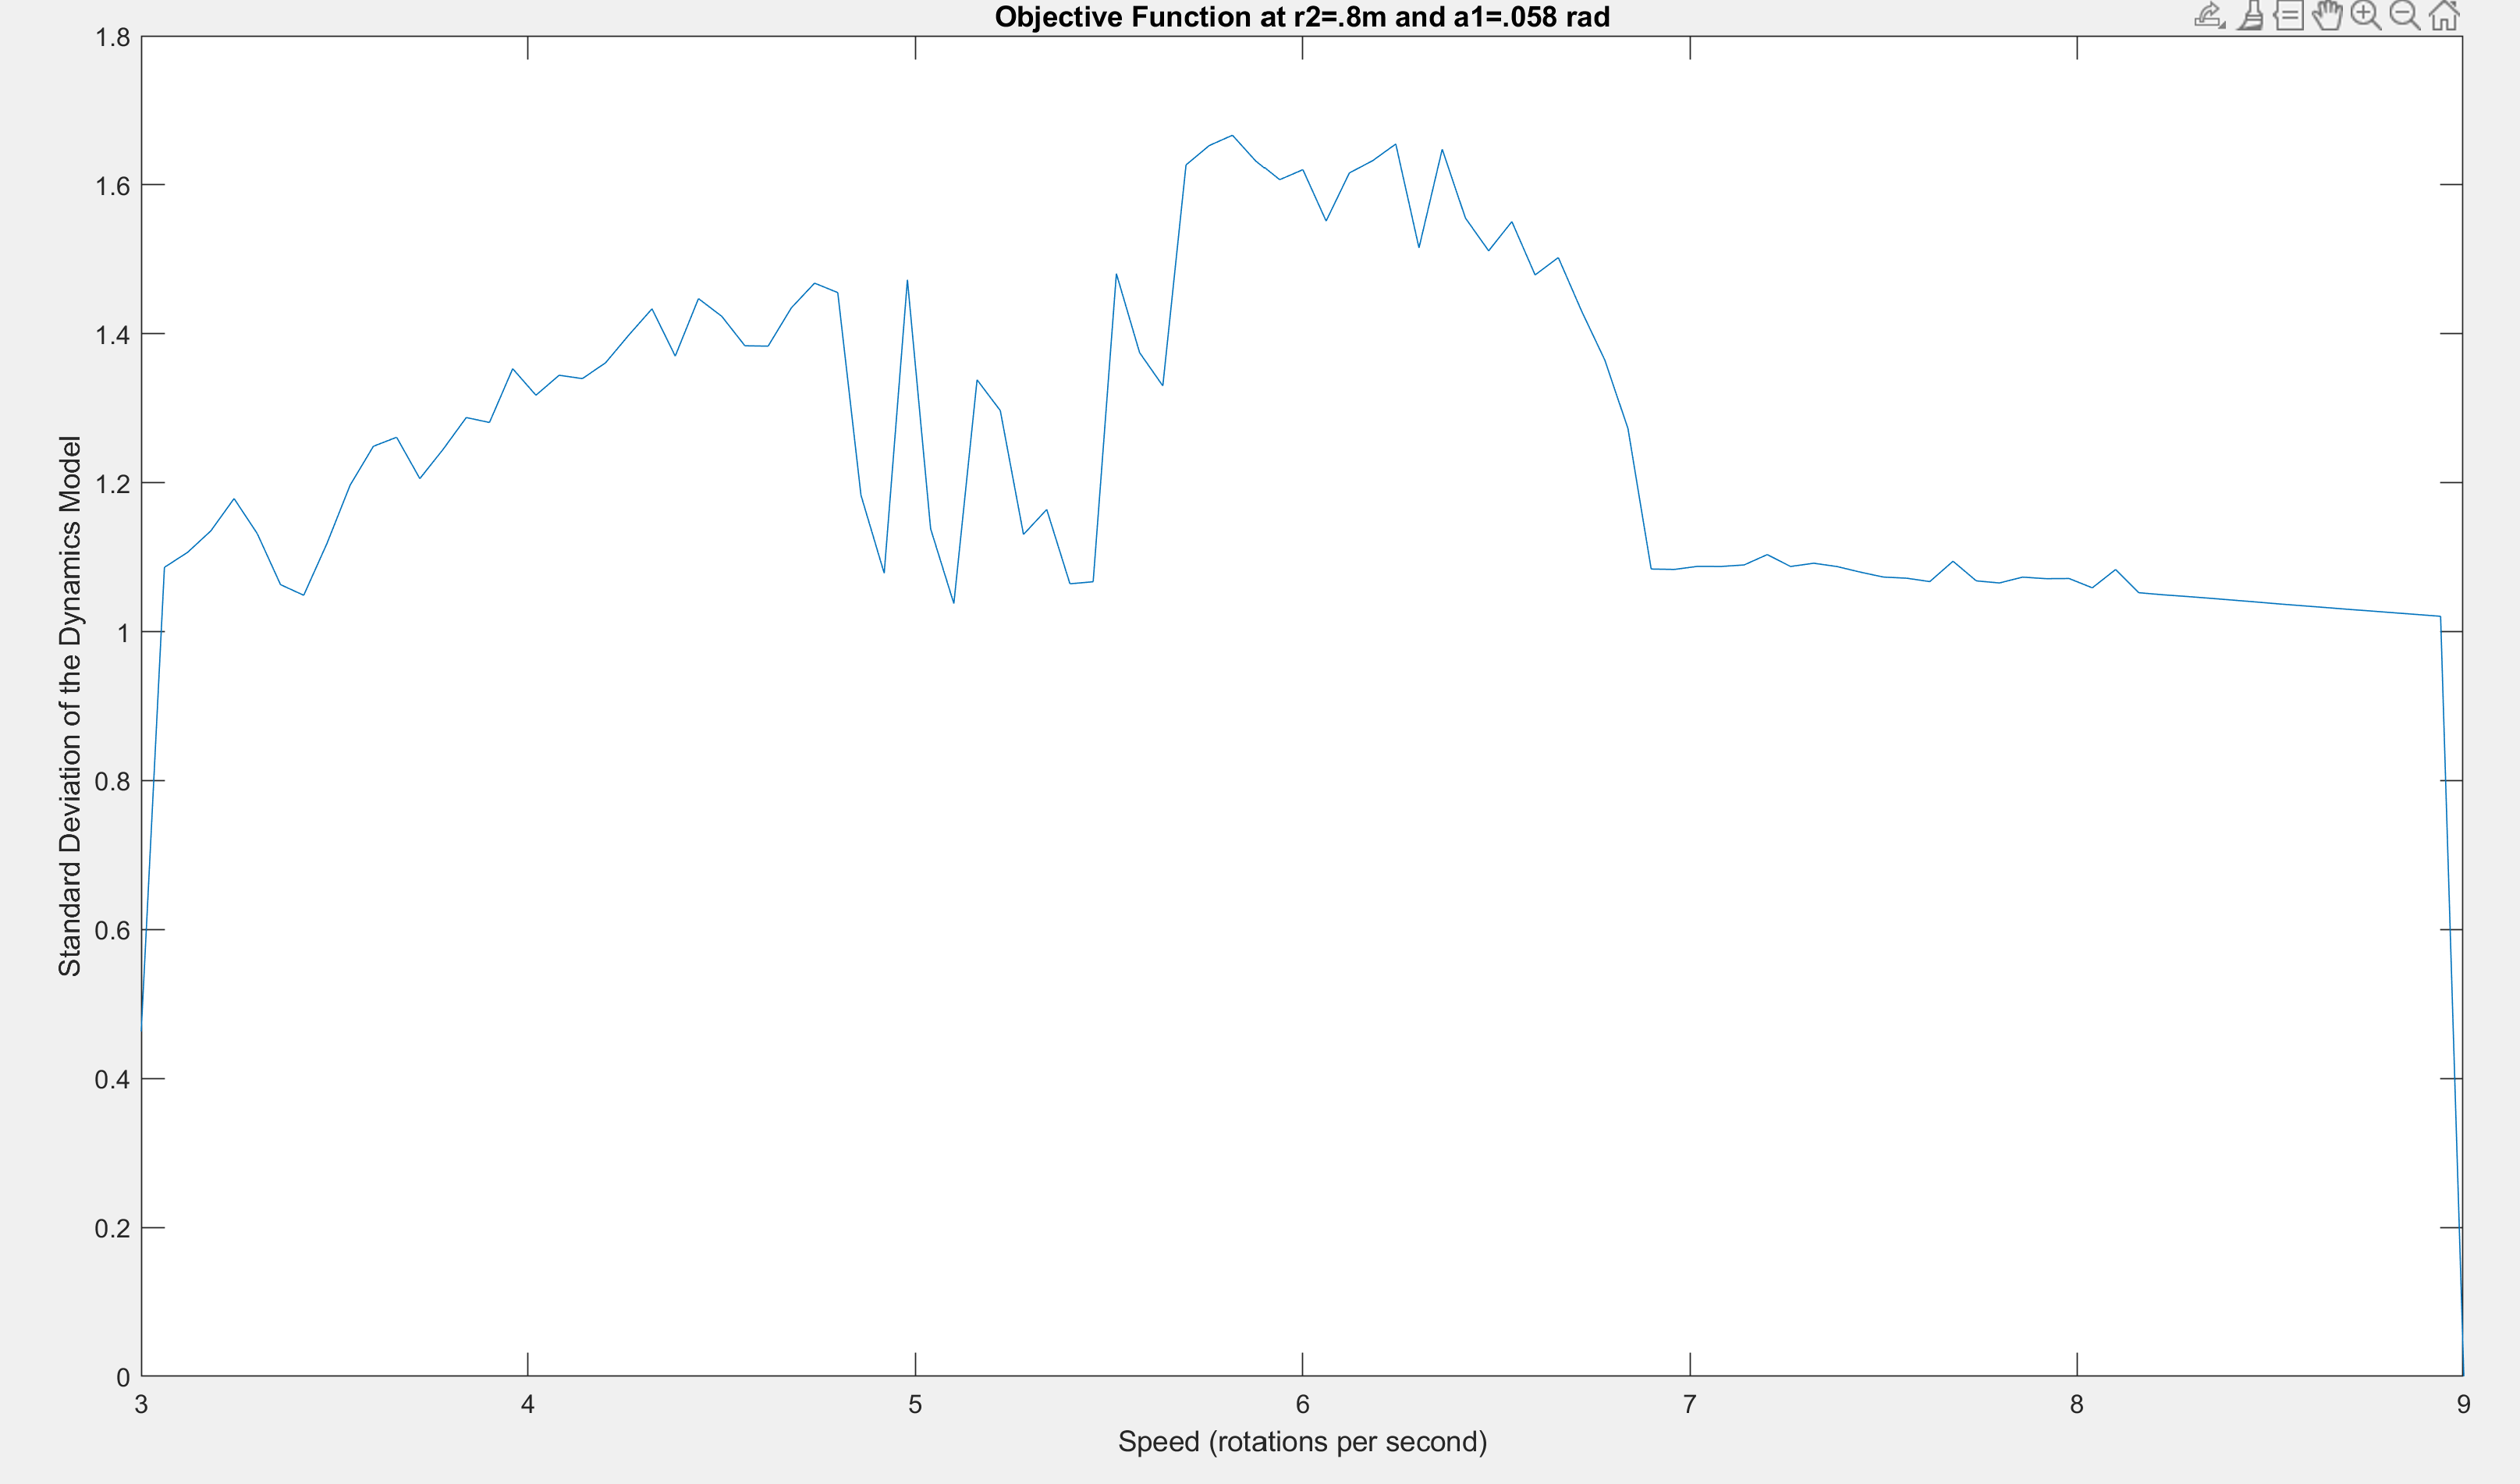
\includegraphics[width=0.75\linewidth]{noopinit.png}
    \caption{ Generated plot of the dynamics standard deviation vs angular velocity  }
    \label{fig:noopinit}
\end{figure}
	\begin{figure}[H]
    \centering
    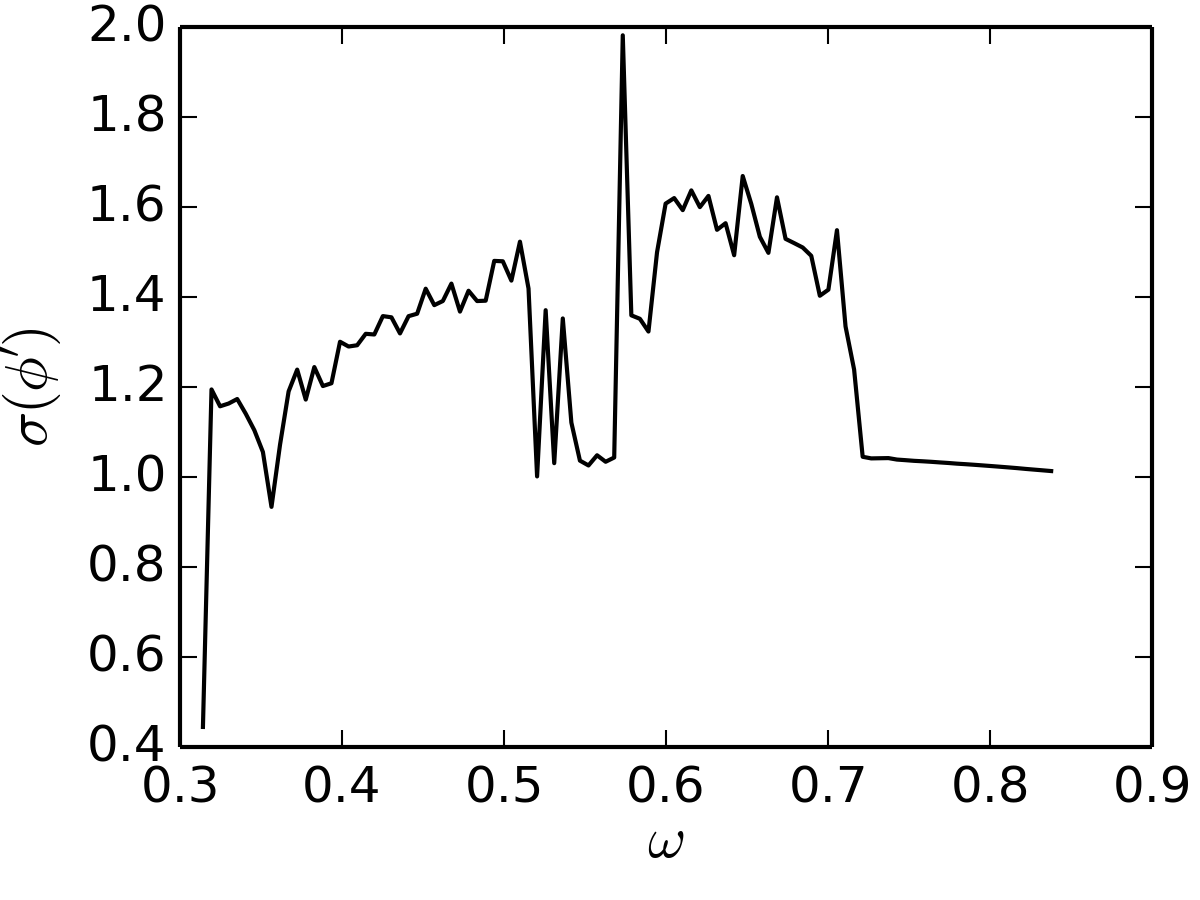
\includegraphics[width=0.5\linewidth]{piazza.png}
    \caption{ Provided plot of the dynamics standard deviation vs angular velocity \cite{piazza}}
    \label{fig:piazza}
\end{figure}
	
A comparison of figures \ref{fig:noopinit} and \ref{fig:piazza} shows that the objective function produces similar results to the provided plot. The broad behavior of both plots show an increase in the standard deviation of the movement to a maximum around of .6 rad/sec (6 rot/sec) before dropping and flatlining around .7 rad/sec (7 rot/sec). This behavior is also similar to the behavior described in \cite{dynamics}.  This makes sense within the context of the problem as when $\omega$ is small the cart doesn't have enough energy to spin erratically. Additionally, when $\omega$ is too large the centripetal acceleration causes the center of mass to be flung outwards harder than the force of gravity can counteract resulting in limited eccentricity.
	
\subsection{Convergence}

The convergence plot shown in figure \ref{fig:conv} was calculated over a range of movement cycles for the design parameters $\omega$=6.5 rot/sec, $\alpha_{1}$=0.058 rad, and $r_{2}$=0.8 m with the same initial states as in the previous section. As is seen in figure \ref{fig:conv} the dynamics function roughly converges to steady state around a value of 1.55 after 700-800 hills, so T=800 hills was chosen for use in optimization.
	\begin{figure}[H]
    \centering
    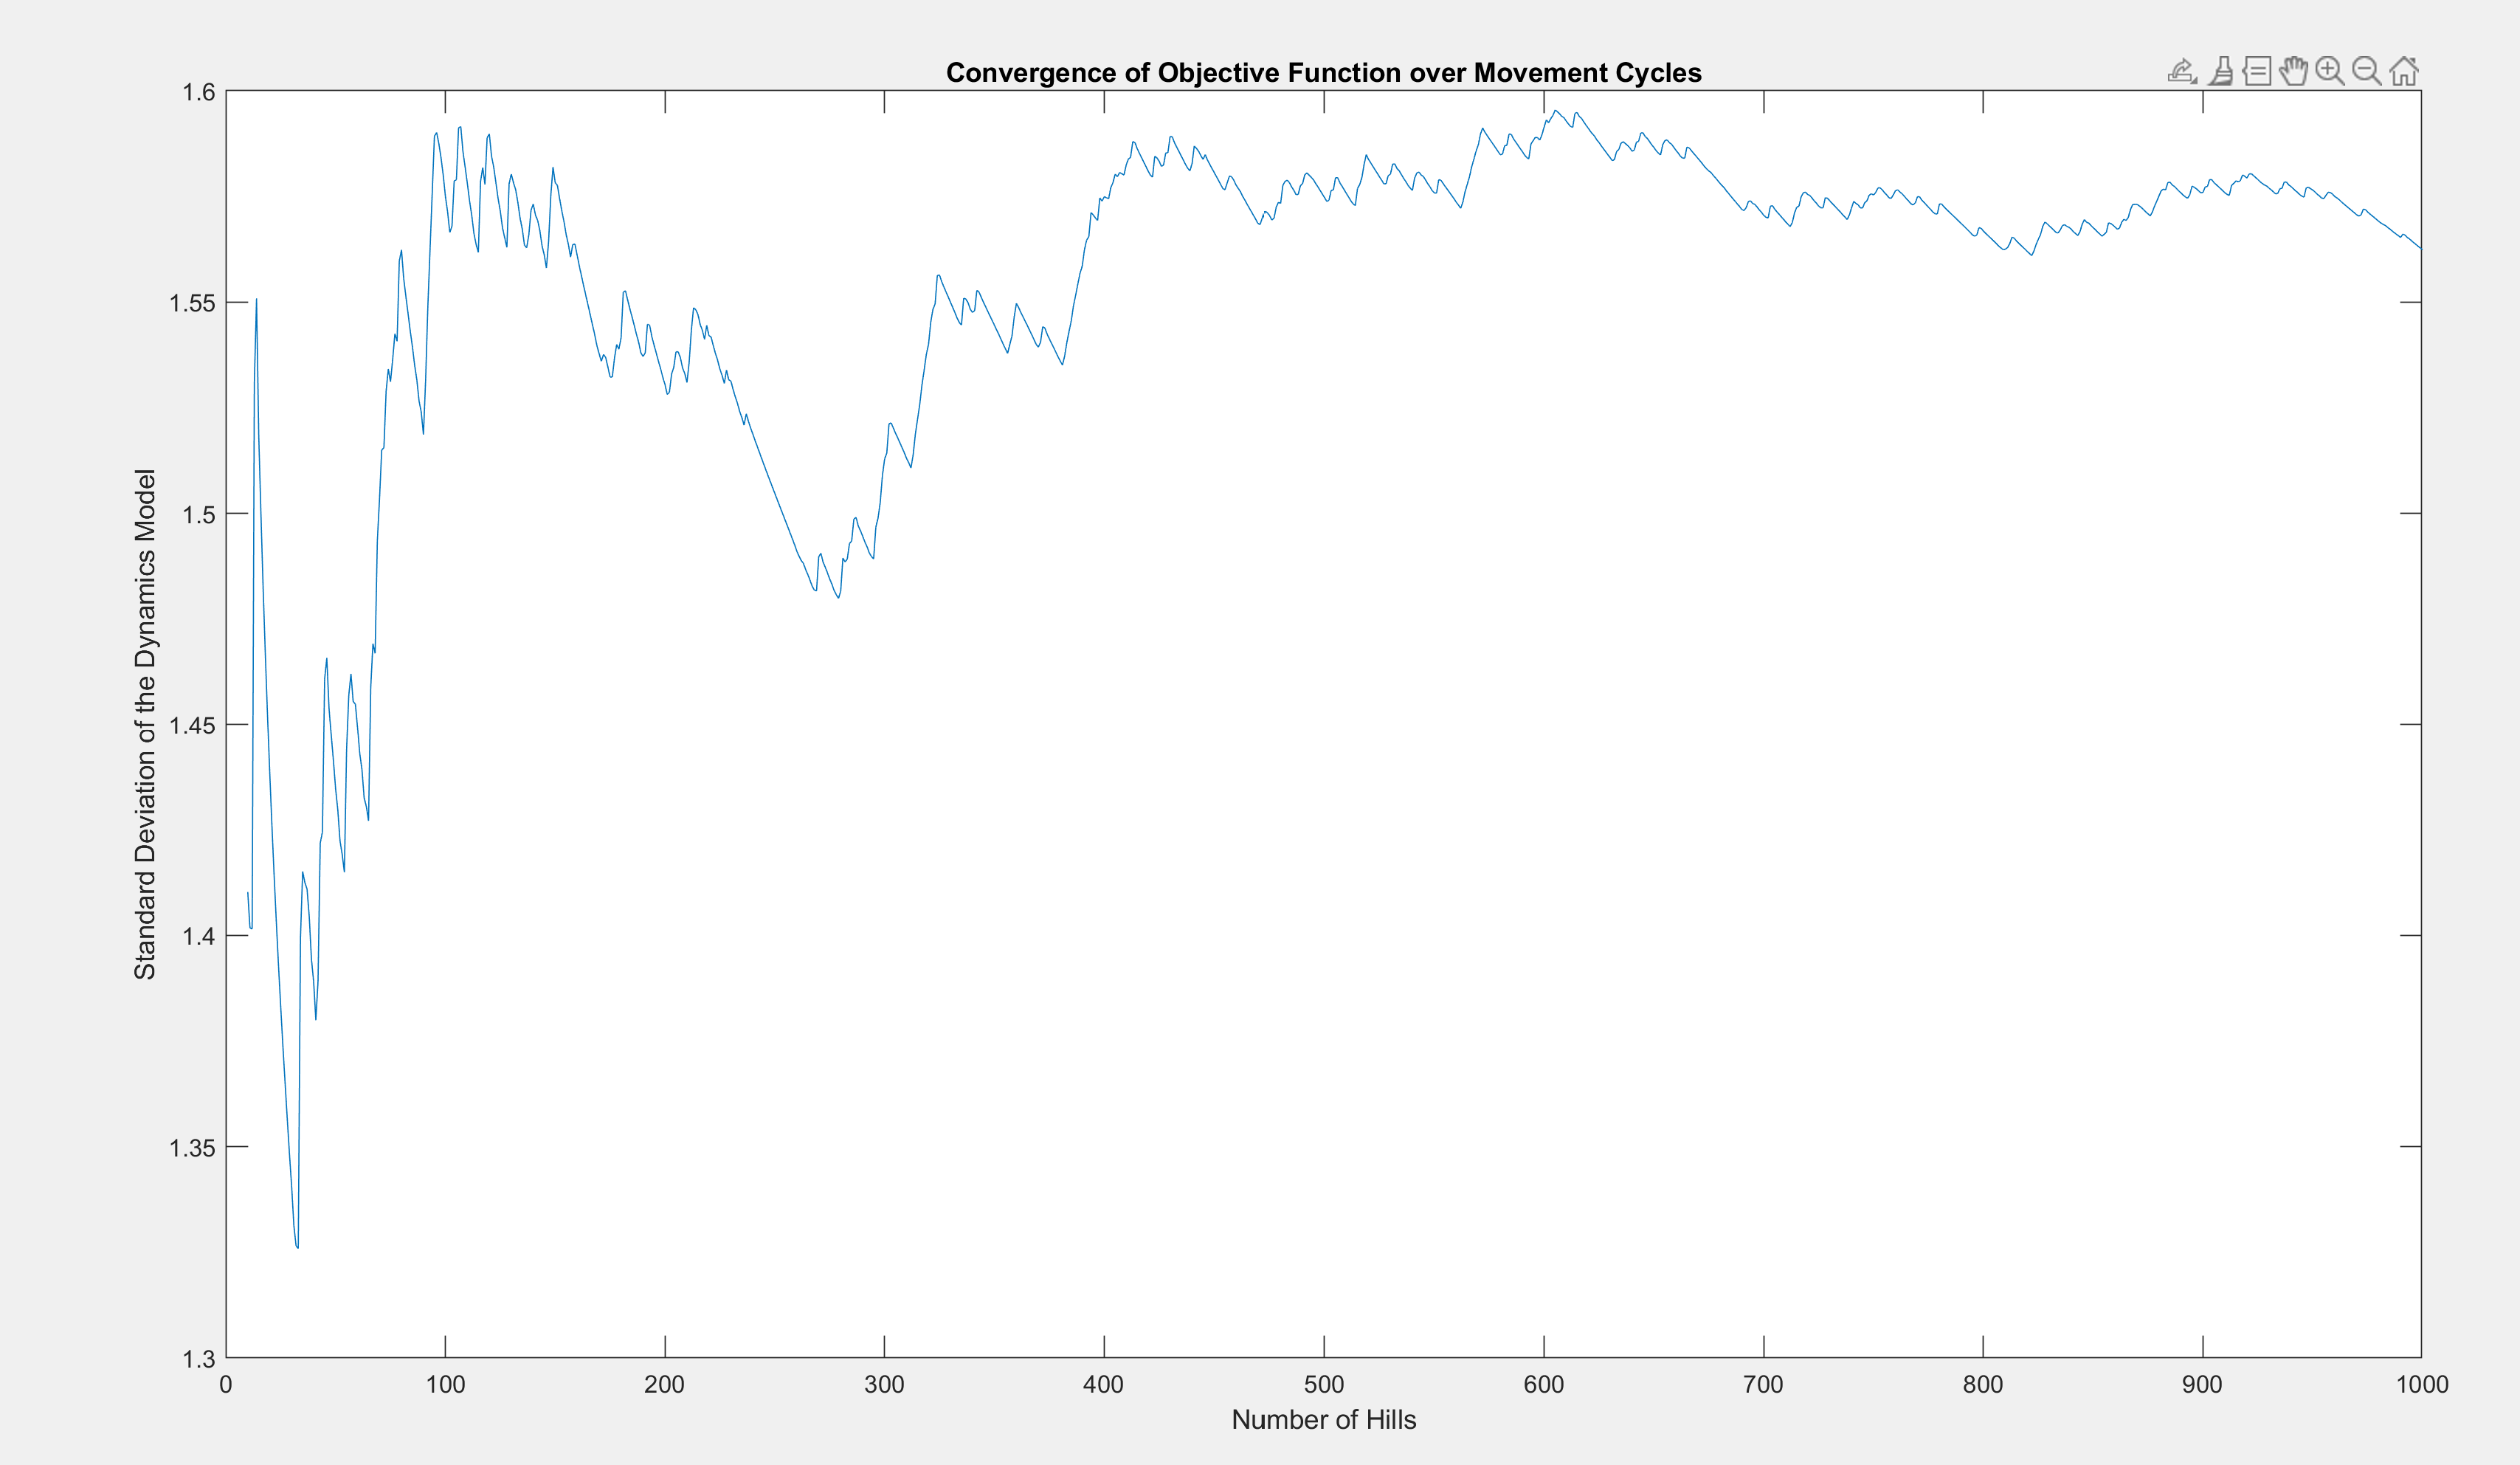
\includegraphics[width=0.75\linewidth]{convergence.png}
    \caption{ Plot of the standard deviation of the model over the number of hills gone over }
    \label{fig:conv}
\end{figure}
\subsection{Optimization Results}

The initial hyper parameters were approximated using the results in \ref{sec:verification} were chosen from the parts of figure \ref{fig:noopinit} as shown in figure \ref{fig:hyper}.

	\begin{figure}[H]
    \centering
    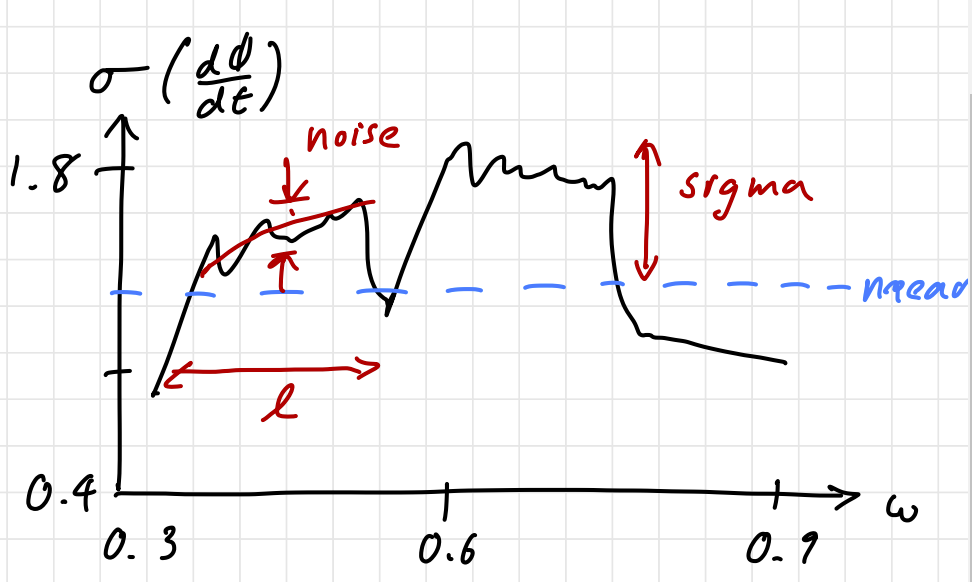
\includegraphics[width=0.75\linewidth]{hyper.png}
    \caption{ Provided drawing for calculating GPML hyper-parameters \cite{lab3notes}}
   \label{fig:hyper}
\end{figure}

All parameters used in the final optimization were adjusted between optimization attempts until a consistent result was reached each time the optimization was run (in a reasonable time) and are shown in table \ref{tab:param}.

\begin{table}[H]
\center
\caption{Design Parameters}
\label{tab:param}
\center
\begin{tabular}{lll}
Parameter                       & Value & Units \\ \hline
noise                           & .4    &       \\
L                               & .4    &       \\
sigma                           & .75   &       \\
T                               & 800   & hills \\
Absolute tolerance              & $5*10^{-2}$ &       \\
Iterative tolerance             & $10^{-9}$  &       \\
Initial $\phi_{1} $                           & $\frac{-\pi}{2}$ & rad   \\
Initial $\phi_{2}   $                         & 0     & rad/s \\
lhssamples                      & 200   &       \\
Maximum Optimization Iterations & 200   &      
\end{tabular}
\end{table}

Slices of the objective function and surrogate models along $\omega$ are shown in figures \ref{fig:opinit} and \ref{fig:finslice} for the nominal and final designs respectively, demonstrating a reasonably good fit to the trends in the objective function. The results of the optimization are summarized in table \ref{tab:results} along with a comparison with the nominal values.
	\begin{figure}[H]
    \centering
    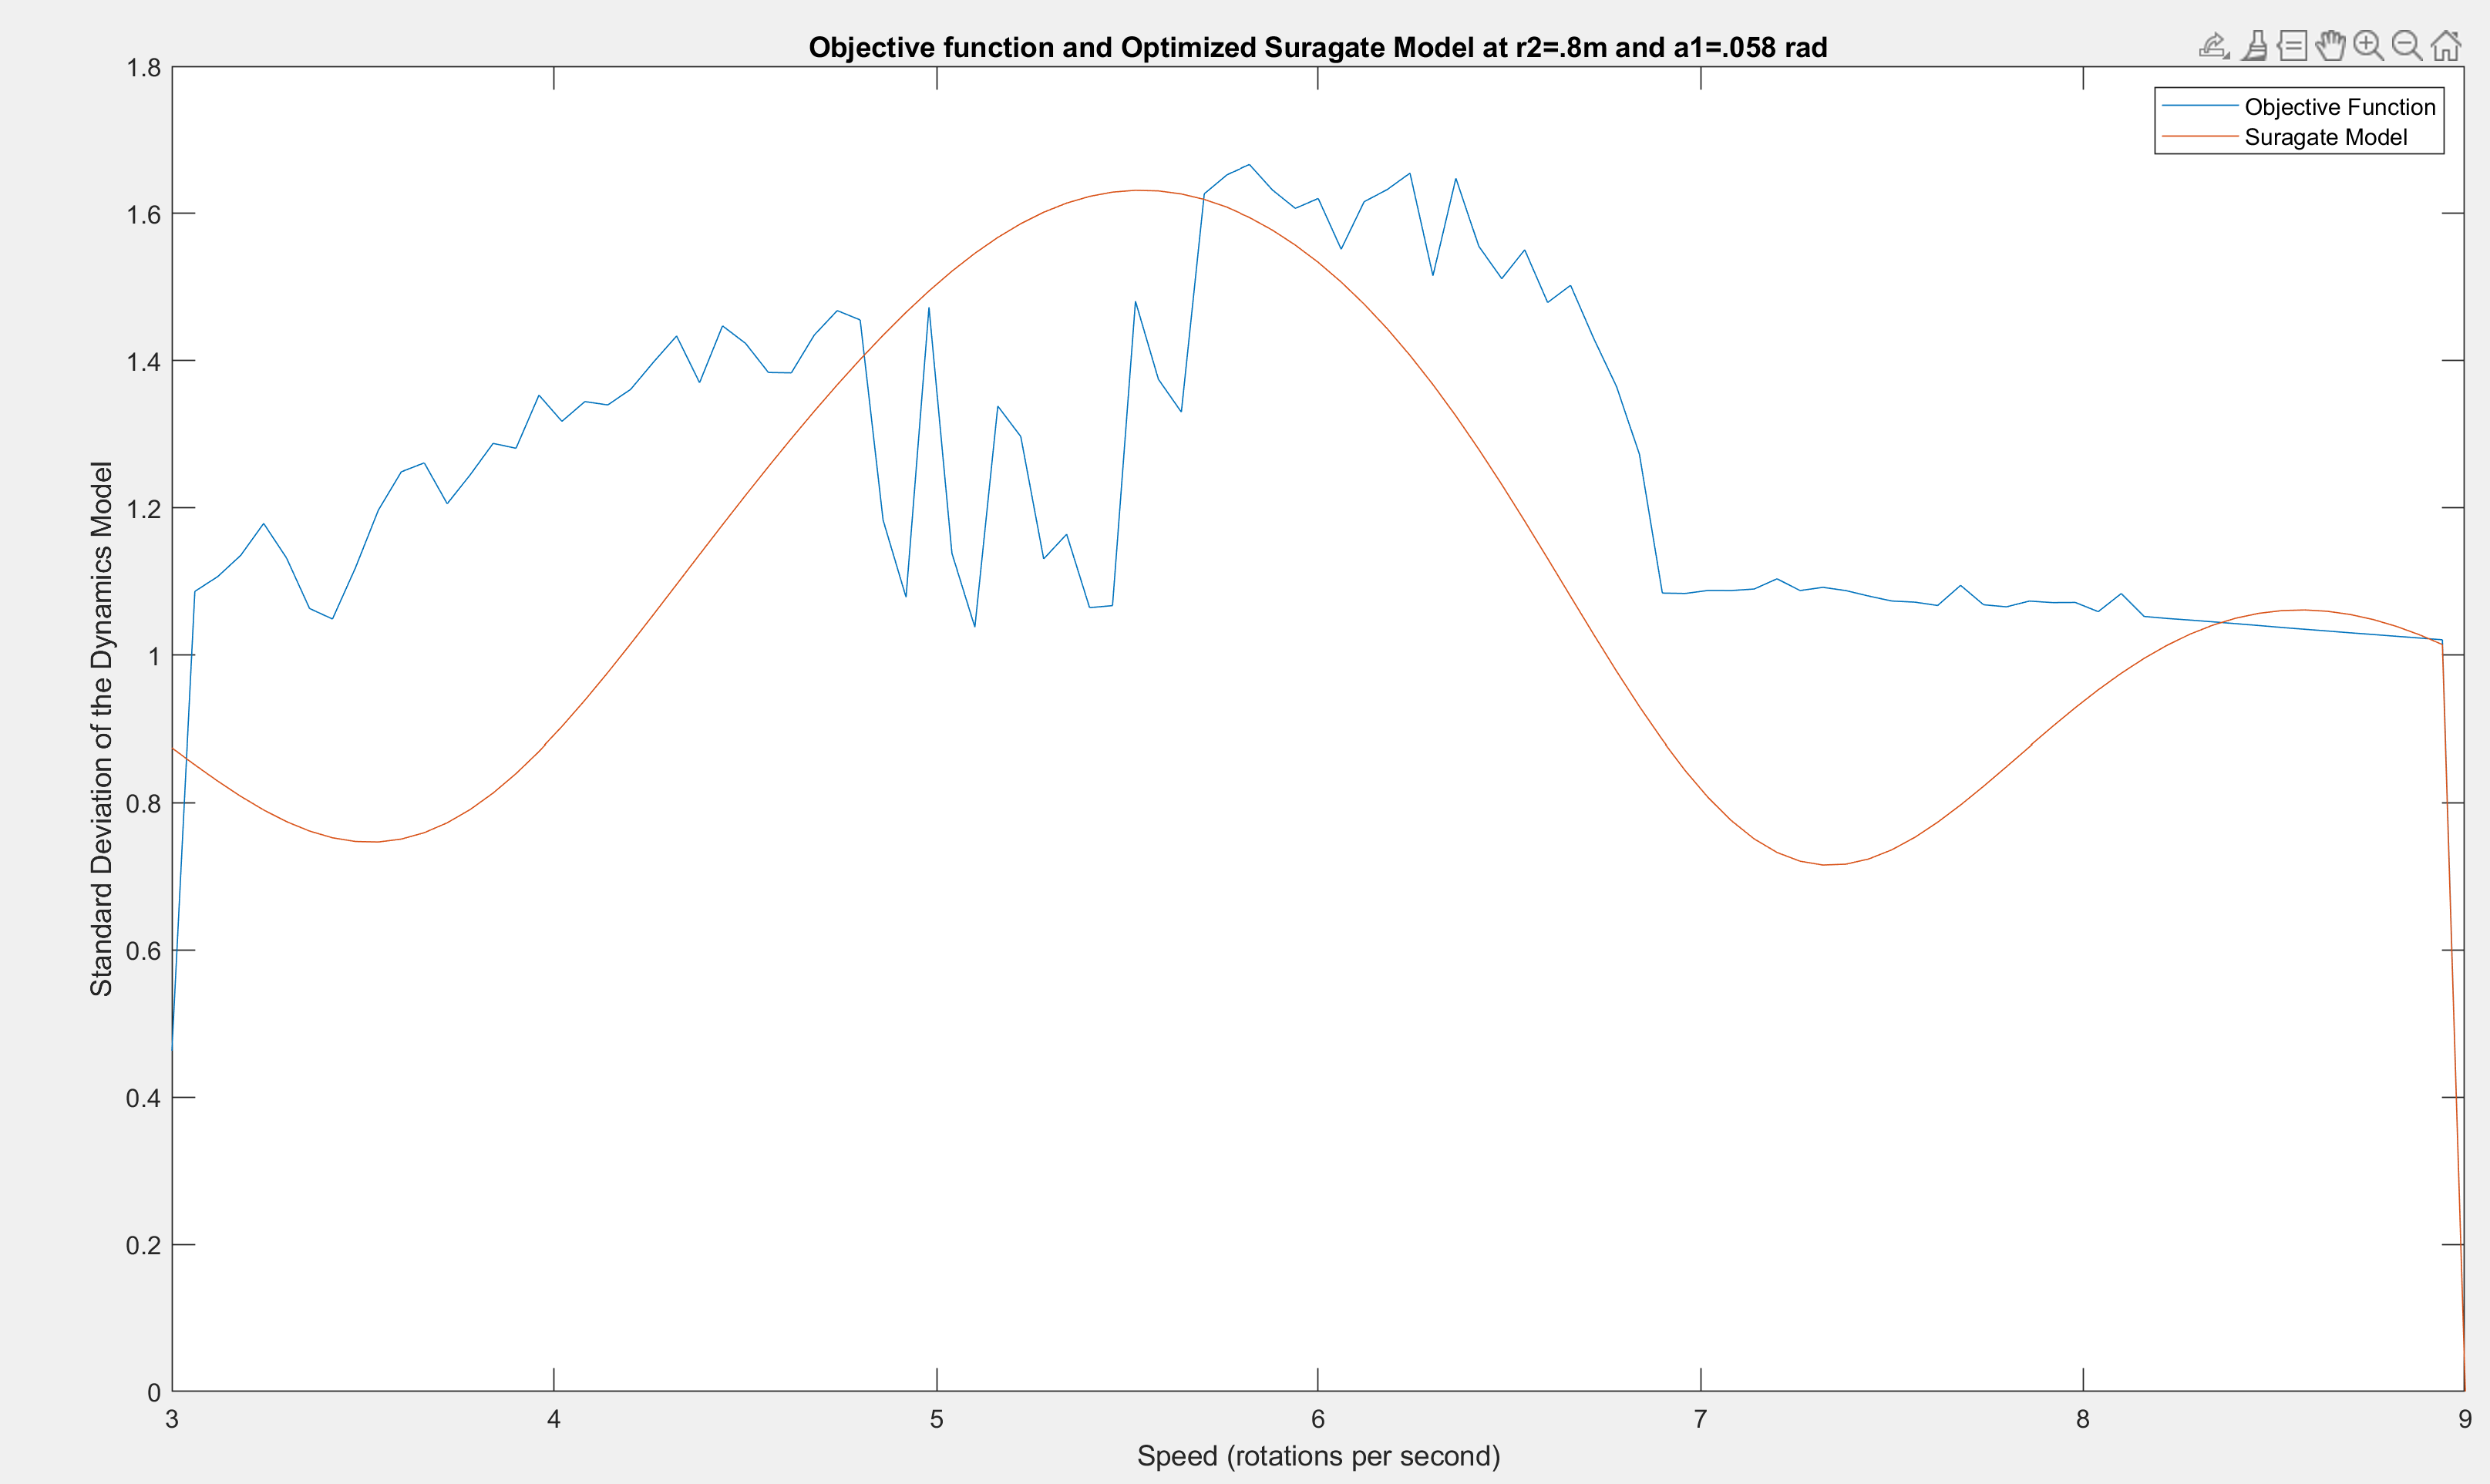
\includegraphics[width=0.75\linewidth]{opinit.png}
    \caption{ Generated plot of the dynamics standard deviation vs angular velocity  }
    \label{fig:opinit}
\end{figure}
\begin{figure}[H]
    \centering
    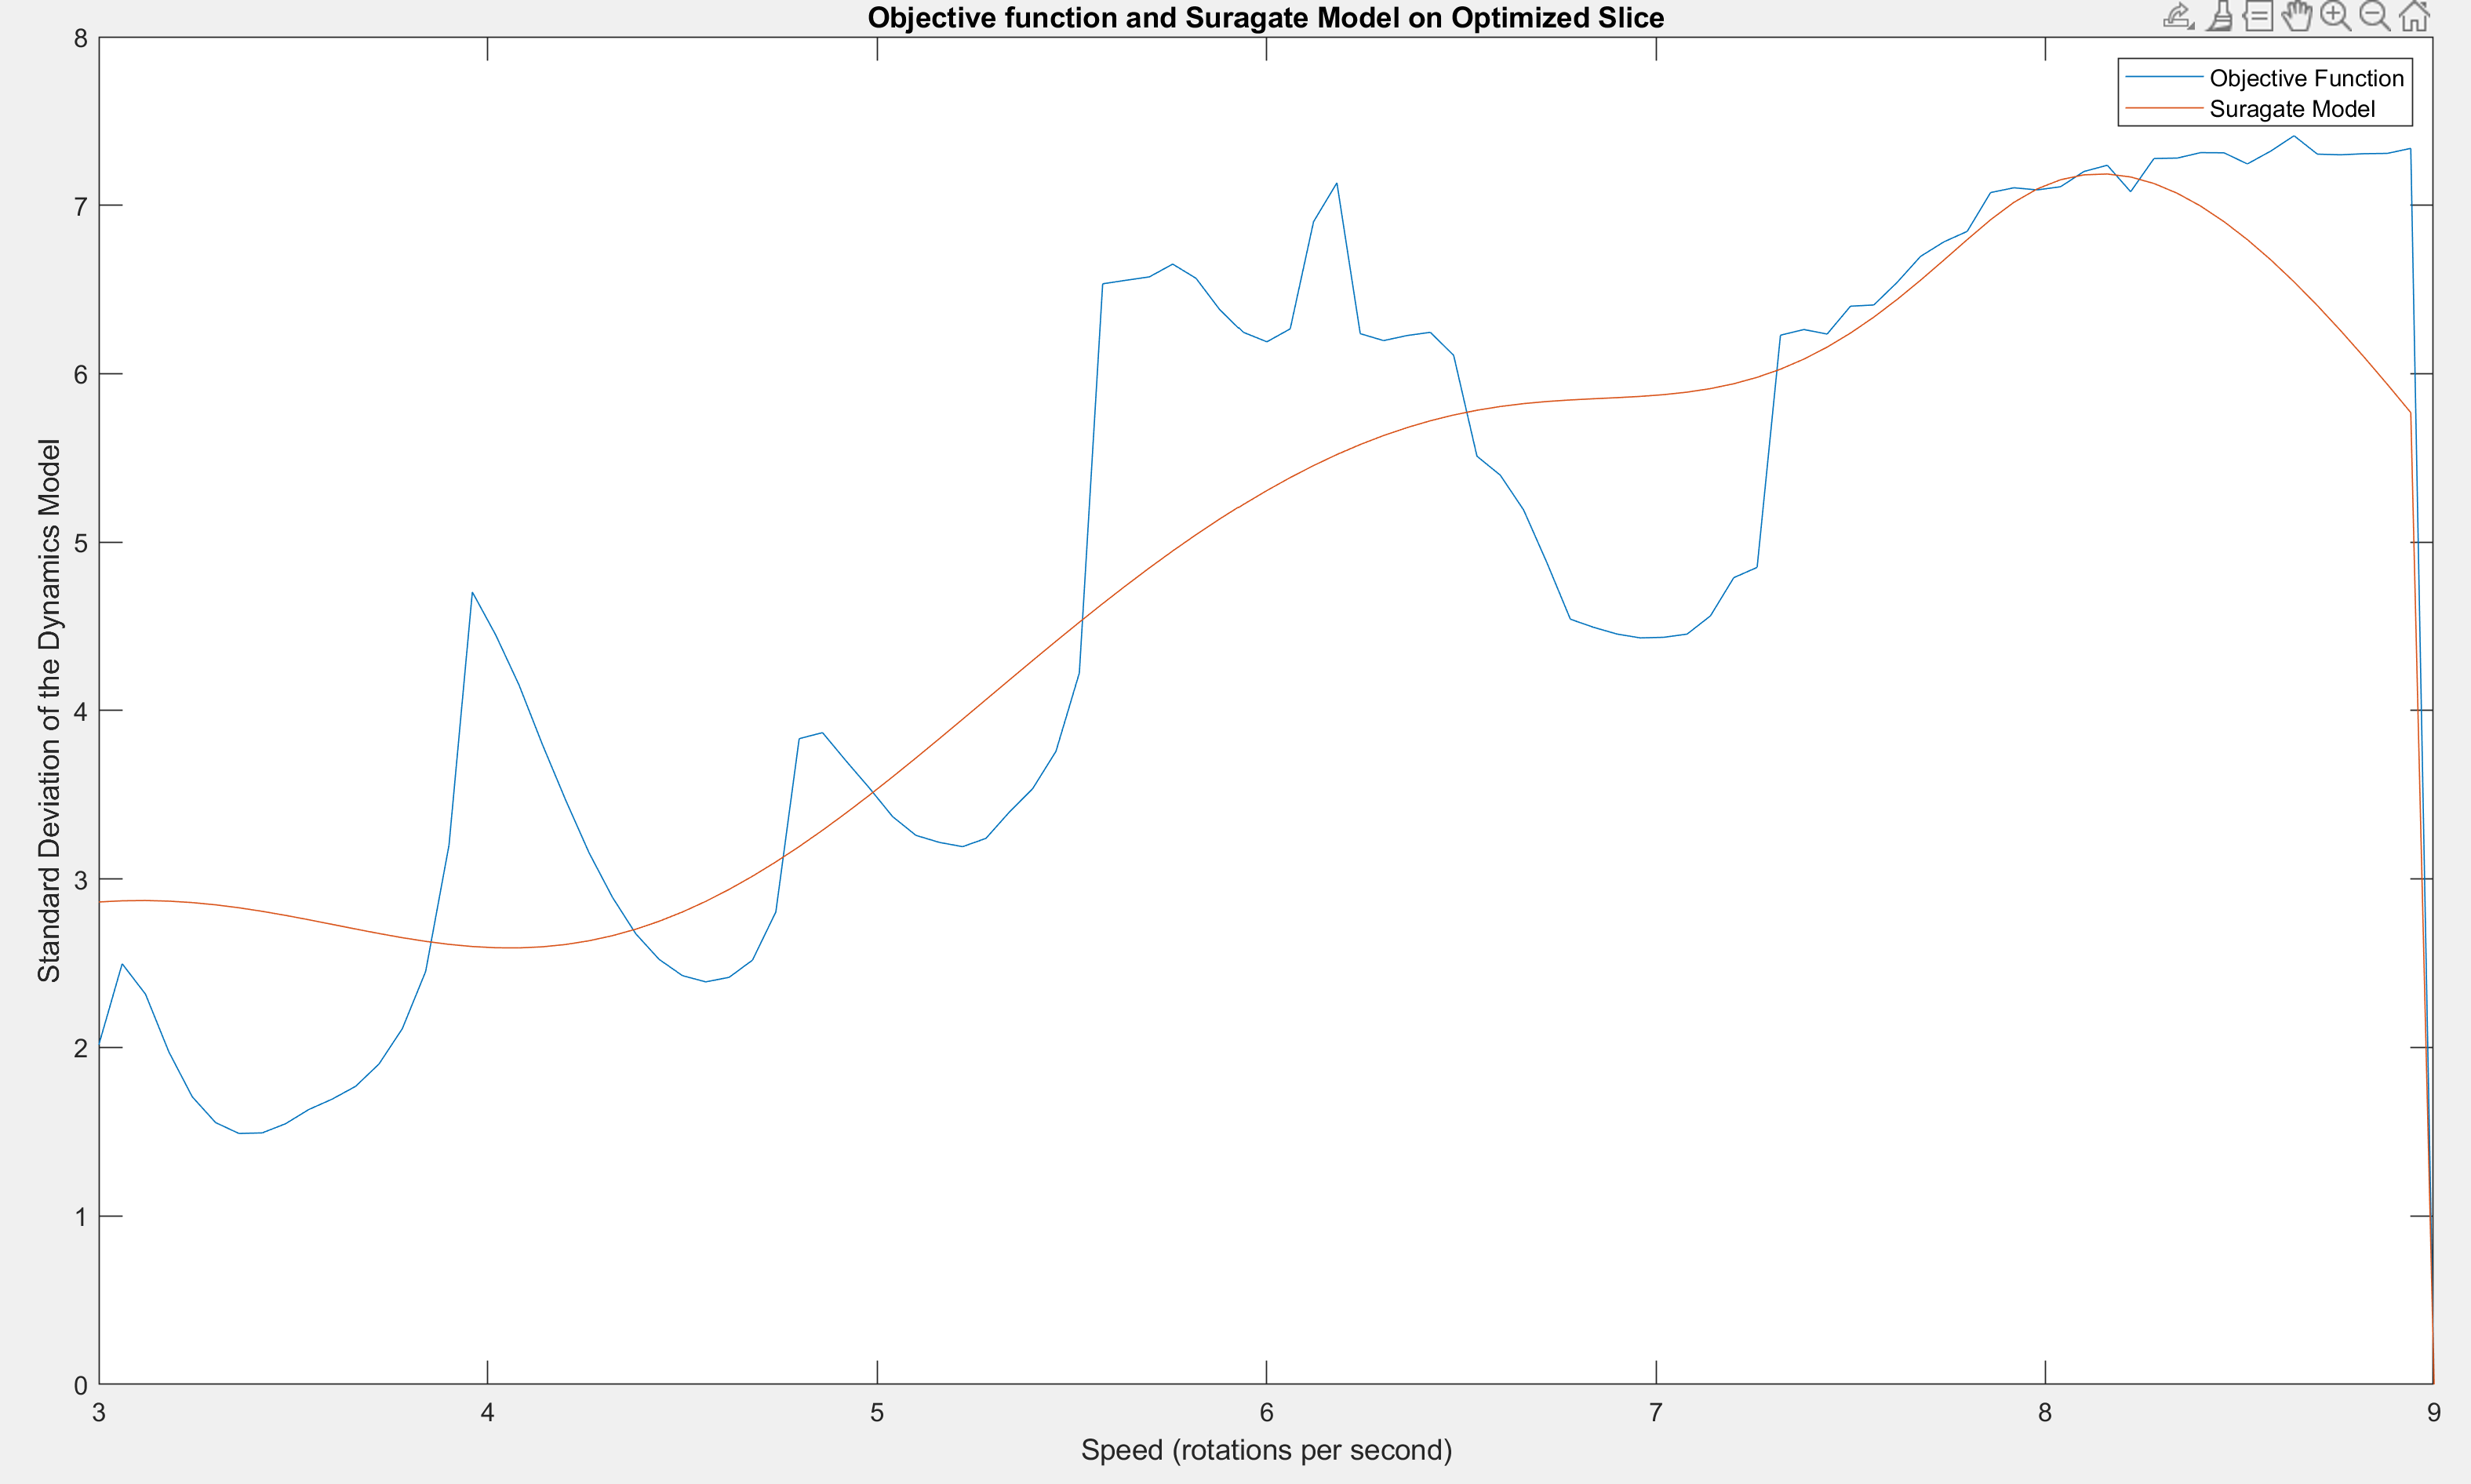
\includegraphics[width=0.75\linewidth]{finslice.png}
    \caption{ Generated plot of the dynamics standard deviation vs angular velocity with final design parameters  }
    \label{fig:finslice}
\end{figure}
	
	\begin{table}[H]
	\caption{Results}
\label{tab:results}
\center
\begin{tabular}{lllll}
Design    & $\omega$ (rot/s) & $\alpha_{1}$ (rad) & $r_{2}$ (m) & Objective Value \\ \hline
Nominal   & 6.5     & 0.058 & 0.8 & 1.5668          \\
Optimized & 8       & 0.3   & 0.1 & 7.1184         
\end{tabular}
\end{table}
	
While the optimization algorithm was running, the iteration outputs were monitered and consistently showed a feasibility score of 0 with a first-order optimality that would decrease at least six orders of magnitude each time \lstinline{fmincon()} was run. The final result of the optimization was a 354 percent increase in the standard deviation of the angular velocity of the cart. 

\medskip

\section{Conclusions}

The implementation of the SQP optimization algorithm with the surrogate model for this lab was successful. The resulting standard deviation represents a 354 percent increase in the standard deviation of the angular velocity of the cart over the nominal parameters while remaining within the problem constraints. The resulting parameters are at the upper bounds of the angular velocity and hill size and the lower bound of the radius. These results make sense because a large hill with a small radius and high speed would cause the cart to spin erratically.

However, these results may not be representative of real implementations. This is because the model had limitations imposed on it by the simplifying assumptions. The assumption of the ride being at steady state through the convergence study was used to limit the effect of the initial states on the results. However, this means that the ride was optimized for a run time exceeding 30 minutes which is unrealistic. Additionally, the dynamics model assumed negligible effects from the riders, which is unrealistic as riders will have a noticeable affect on the location of the center of mass and will likely move during the ride. 

 Basic optimization algorithms, such as the ones used in this lab, can be powerful tools for understanding the complex interactions between different design variables in engineering design problems and balancing the design variables to arrive at an optimal solution. Understanding how to extend optimization algorithms to problems that are too noisy for them to efficiently solve through the use of surrogate models. Knowing how these algorithms work and the trade-offs between accuracy and run time is important when using these optimization algorithms and surrogate models together to solve problems. 

\addcontentsline{toc}{section}{References}
\printbibliography
\newpage
\section{Appendix}

\lstset{language=Matlab,%
    %basicstyle=\color{red},
    breaklines=true,%
    morekeywords={matlab2tikz},
    keywordstyle=\color{blue},%
    morekeywords=[2]{1}, keywordstyle=[2]{\color{black}},
    identifierstyle=\color{black},%
    stringstyle=\color{mylilas},
    commentstyle=\color{mygreen},%
    showstringspaces=false,%without this there will be a symbol in the places where there is a space
    numbers=left,%
    numberstyle={\tiny \color{black}},% size of the numbers
    numbersep=9pt, % this defines how far the numbers are from the text
    emph=[1]{for,end,break},emphstyle=[1]\color{red}, %some words to emphasise
    %emph=[2]{word1,word2}, emphstyle=[2]{style},    
}
\subsection{dynamics.m}
\label{sec:dynamics}
\lstinputlisting{dynamics.m}
\newpage
\subsection{obj.m}
\label{sec:obj}
\lstinputlisting{obj.m}
\newpage
\subsection{run.m}
\label{sec:run}
\lstinputlisting{run.m}
\newpage
\subsection{plots.m}
\label{sec:plots}
\lstinputlisting{plots.m}
\subsection{fmincon Output}
\label{sec:fincon}
\begin{figure}[H]
    \centering
    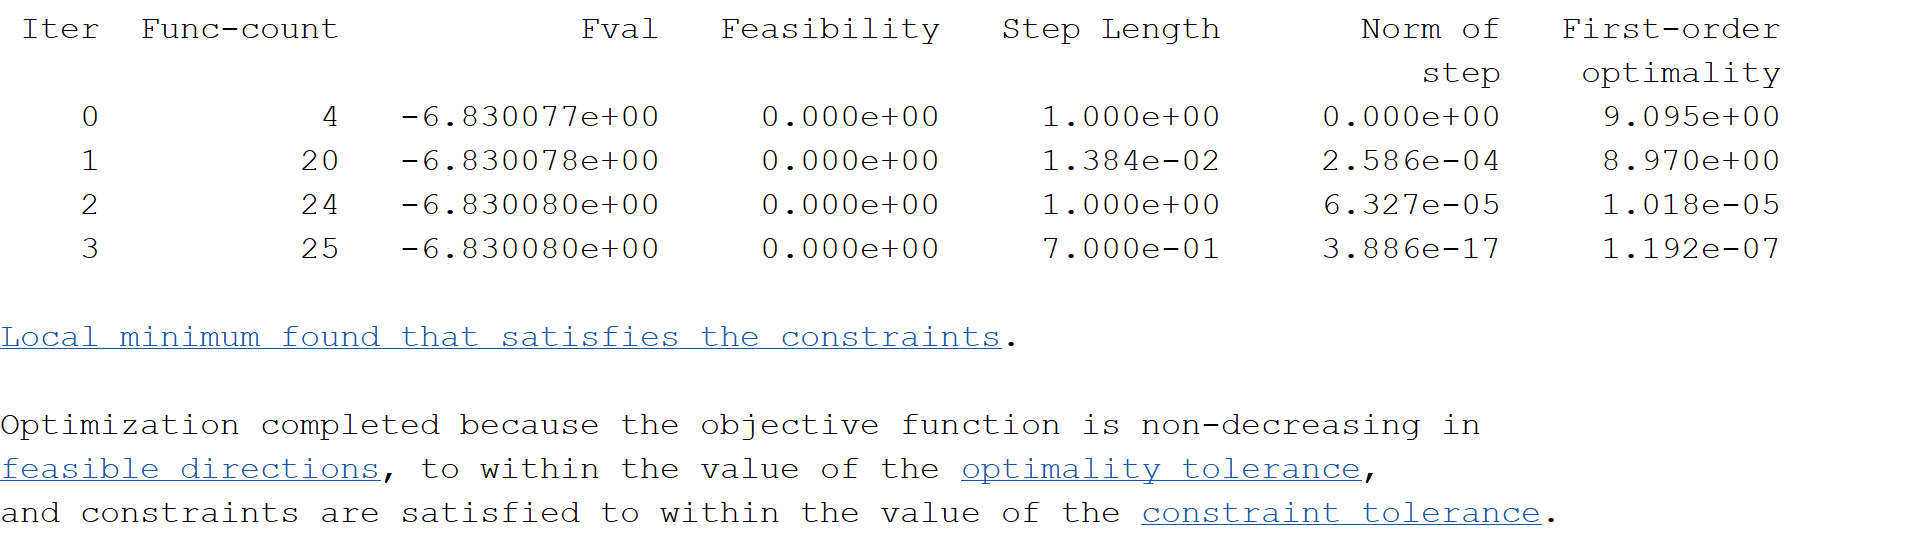
\includegraphics[width=0.75\linewidth]{fminconoutput.png}
    \caption{ Example outpt of fmincon }
    \label{fig:fmincon}
\end{figure}

\end{document}